% Options for packages loaded elsewhere
\PassOptionsToPackage{unicode}{hyperref}
\PassOptionsToPackage{hyphens}{url}
%
\documentclass[
]{article}
\usepackage{amsmath,amssymb}
\usepackage{lmodern}
\usepackage{ifxetex,ifluatex}
\ifnum 0\ifxetex 1\fi\ifluatex 1\fi=0 % if pdftex
  \usepackage[T1]{fontenc}
  \usepackage[utf8]{inputenc}
  \usepackage{textcomp} % provide euro and other symbols
\else % if luatex or xetex
  \usepackage{unicode-math}
  \defaultfontfeatures{Scale=MatchLowercase}
  \defaultfontfeatures[\rmfamily]{Ligatures=TeX,Scale=1}
\fi
% Use upquote if available, for straight quotes in verbatim environments
\IfFileExists{upquote.sty}{\usepackage{upquote}}{}
\IfFileExists{microtype.sty}{% use microtype if available
  \usepackage[]{microtype}
  \UseMicrotypeSet[protrusion]{basicmath} % disable protrusion for tt fonts
}{}
\makeatletter
\@ifundefined{KOMAClassName}{% if non-KOMA class
  \IfFileExists{parskip.sty}{%
    \usepackage{parskip}
  }{% else
    \setlength{\parindent}{0pt}
    \setlength{\parskip}{6pt plus 2pt minus 1pt}}
}{% if KOMA class
  \KOMAoptions{parskip=half}}
\makeatother
\usepackage{xcolor}
\IfFileExists{xurl.sty}{\usepackage{xurl}}{} % add URL line breaks if available
\IfFileExists{bookmark.sty}{\usepackage{bookmark}}{\usepackage{hyperref}}
\hypersetup{
  pdftitle={Final Project: Water Absorption in Hardwoods},
  pdfauthor={Jacob Nelson, Megan Hawley, Emily Groves, Clayton Jannusch, Gavin Wilson},
  hidelinks,
  pdfcreator={LaTeX via pandoc}}
\urlstyle{same} % disable monospaced font for URLs
\usepackage[margin=1in]{geometry}
\usepackage{color}
\usepackage{fancyvrb}
\newcommand{\VerbBar}{|}
\newcommand{\VERB}{\Verb[commandchars=\\\{\}]}
\DefineVerbatimEnvironment{Highlighting}{Verbatim}{commandchars=\\\{\}}
% Add ',fontsize=\small' for more characters per line
\usepackage{framed}
\definecolor{shadecolor}{RGB}{248,248,248}
\newenvironment{Shaded}{\begin{snugshade}}{\end{snugshade}}
\newcommand{\AlertTok}[1]{\textcolor[rgb]{0.94,0.16,0.16}{#1}}
\newcommand{\AnnotationTok}[1]{\textcolor[rgb]{0.56,0.35,0.01}{\textbf{\textit{#1}}}}
\newcommand{\AttributeTok}[1]{\textcolor[rgb]{0.77,0.63,0.00}{#1}}
\newcommand{\BaseNTok}[1]{\textcolor[rgb]{0.00,0.00,0.81}{#1}}
\newcommand{\BuiltInTok}[1]{#1}
\newcommand{\CharTok}[1]{\textcolor[rgb]{0.31,0.60,0.02}{#1}}
\newcommand{\CommentTok}[1]{\textcolor[rgb]{0.56,0.35,0.01}{\textit{#1}}}
\newcommand{\CommentVarTok}[1]{\textcolor[rgb]{0.56,0.35,0.01}{\textbf{\textit{#1}}}}
\newcommand{\ConstantTok}[1]{\textcolor[rgb]{0.00,0.00,0.00}{#1}}
\newcommand{\ControlFlowTok}[1]{\textcolor[rgb]{0.13,0.29,0.53}{\textbf{#1}}}
\newcommand{\DataTypeTok}[1]{\textcolor[rgb]{0.13,0.29,0.53}{#1}}
\newcommand{\DecValTok}[1]{\textcolor[rgb]{0.00,0.00,0.81}{#1}}
\newcommand{\DocumentationTok}[1]{\textcolor[rgb]{0.56,0.35,0.01}{\textbf{\textit{#1}}}}
\newcommand{\ErrorTok}[1]{\textcolor[rgb]{0.64,0.00,0.00}{\textbf{#1}}}
\newcommand{\ExtensionTok}[1]{#1}
\newcommand{\FloatTok}[1]{\textcolor[rgb]{0.00,0.00,0.81}{#1}}
\newcommand{\FunctionTok}[1]{\textcolor[rgb]{0.00,0.00,0.00}{#1}}
\newcommand{\ImportTok}[1]{#1}
\newcommand{\InformationTok}[1]{\textcolor[rgb]{0.56,0.35,0.01}{\textbf{\textit{#1}}}}
\newcommand{\KeywordTok}[1]{\textcolor[rgb]{0.13,0.29,0.53}{\textbf{#1}}}
\newcommand{\NormalTok}[1]{#1}
\newcommand{\OperatorTok}[1]{\textcolor[rgb]{0.81,0.36,0.00}{\textbf{#1}}}
\newcommand{\OtherTok}[1]{\textcolor[rgb]{0.56,0.35,0.01}{#1}}
\newcommand{\PreprocessorTok}[1]{\textcolor[rgb]{0.56,0.35,0.01}{\textit{#1}}}
\newcommand{\RegionMarkerTok}[1]{#1}
\newcommand{\SpecialCharTok}[1]{\textcolor[rgb]{0.00,0.00,0.00}{#1}}
\newcommand{\SpecialStringTok}[1]{\textcolor[rgb]{0.31,0.60,0.02}{#1}}
\newcommand{\StringTok}[1]{\textcolor[rgb]{0.31,0.60,0.02}{#1}}
\newcommand{\VariableTok}[1]{\textcolor[rgb]{0.00,0.00,0.00}{#1}}
\newcommand{\VerbatimStringTok}[1]{\textcolor[rgb]{0.31,0.60,0.02}{#1}}
\newcommand{\WarningTok}[1]{\textcolor[rgb]{0.56,0.35,0.01}{\textbf{\textit{#1}}}}
\usepackage{graphicx}
\makeatletter
\def\maxwidth{\ifdim\Gin@nat@width>\linewidth\linewidth\else\Gin@nat@width\fi}
\def\maxheight{\ifdim\Gin@nat@height>\textheight\textheight\else\Gin@nat@height\fi}
\makeatother
% Scale images if necessary, so that they will not overflow the page
% margins by default, and it is still possible to overwrite the defaults
% using explicit options in \includegraphics[width, height, ...]{}
\setkeys{Gin}{width=\maxwidth,height=\maxheight,keepaspectratio}
% Set default figure placement to htbp
\makeatletter
\def\fps@figure{htbp}
\makeatother
\setlength{\emergencystretch}{3em} % prevent overfull lines
\providecommand{\tightlist}{%
  \setlength{\itemsep}{0pt}\setlength{\parskip}{0pt}}
\setcounter{secnumdepth}{-\maxdimen} % remove section numbering
\ifluatex
  \usepackage{selnolig}  % disable illegal ligatures
\fi

\title{Final Project: Water Absorption in Hardwoods}
\author{Jacob Nelson, Megan Hawley, Emily Groves, Clayton Jannusch,
Gavin Wilson}
\date{4/10/2022}

\begin{document}
\maketitle

\hypertarget{introduction}{%
\subsection{Introduction}\label{introduction}}

A natural and sustainable building material, softwood has a variety of
uses in construction and engineering. In order to advance building
practices, we seek variation in moisture content of softwoods after
water exposure. Softwood is hygroscopic, meaning it takes on water from
its surrounding environment. The moisture content of wood impacts the
viability of use in various projects. In this paper we will explore the
question: what type of wood absorbs the most water? We will measure the
absorption capabilities of wood by weighing the wood before and after
leaving it submerged in water for a predetermined period of time.
Controllable explanatory variables that will affect this outcome include
type of wood, density of wood, temperature of the water, and length of
time in the water. Uncontrollable explanatory variables that will have
an effect on our measurements include the pH of water, dissolved
materials in the water, time since the wood was harvested, and possible
dissolving of the wood in the water. In the case of the wood dissolving,
we are assuming that because the wood will only be submerged for a short
amount of time, any dissolving that occurs will be negligible. Other
factors can be seen in the fishbone diagram below.

\begin{figure}

{\centering 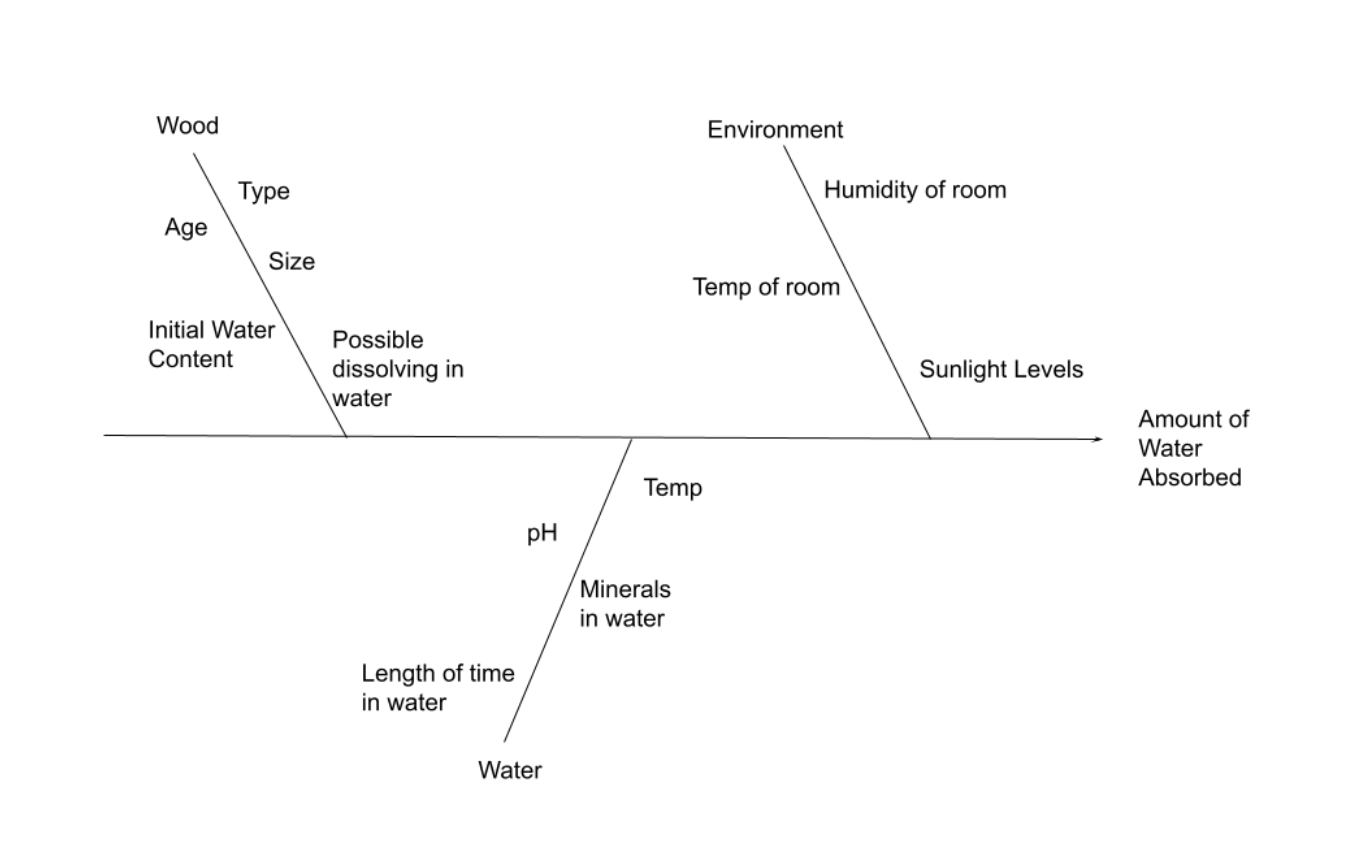
\includegraphics[width=0.8\linewidth]{fishbone} 

}

\caption{Cause and effect fishbone diagram}\label{fig:unnamed-chunk-1}
\end{figure}

Various analyses have been performed on moisture content and the
relation to wood samples. Our team wanted to add to this by studying the
moisture content of various common softwood and hardwood samples after
exposure to water. While we predict the mass of each wood sample will
increase after water exposure, we would like to perform an analysis of
variance of the sample moisture content. Our measurement of interest is
moisture content, is operationally defined as

For each of our wood types, we define a sample mean of for each of our
samples. This leads us to our set of hypotheses:

\(H_0: \mu_{Cherry} = \mu_{Walnut} = \mu_{Ash} = \mu_{Whitebirch} = \mu_{Pine}\)

\(H_A: \mu_{type} \ne \mu_{diffType}\) for at least two woods in the
sample.

To test our hypotheses, we will use a one-way ANOVA, as well as Tukey's
HSD method.

Before any experimentation, we decided as a group to use
\(\alpha = 0.01\)

\hypertarget{methods}{%
\subsection{Methods}\label{methods}}

Design justification-

We intend to use a one way analysis of variance. While deciding on the
parameters of the experiment, resources, available environment, and time
were all limiting factors. Using a one way analysis of various allows
for us to compare moisture content of various wood types while keeping
other variables constant. We will run our five wood samples with four
replicates. The decision to analyze five types of wood was constrained
by the resources available to us. Further, our choice to replicate each
wood type four times was made to maximize replicates while using the
space and resources we had available to us.

\begin{figure}

{\centering 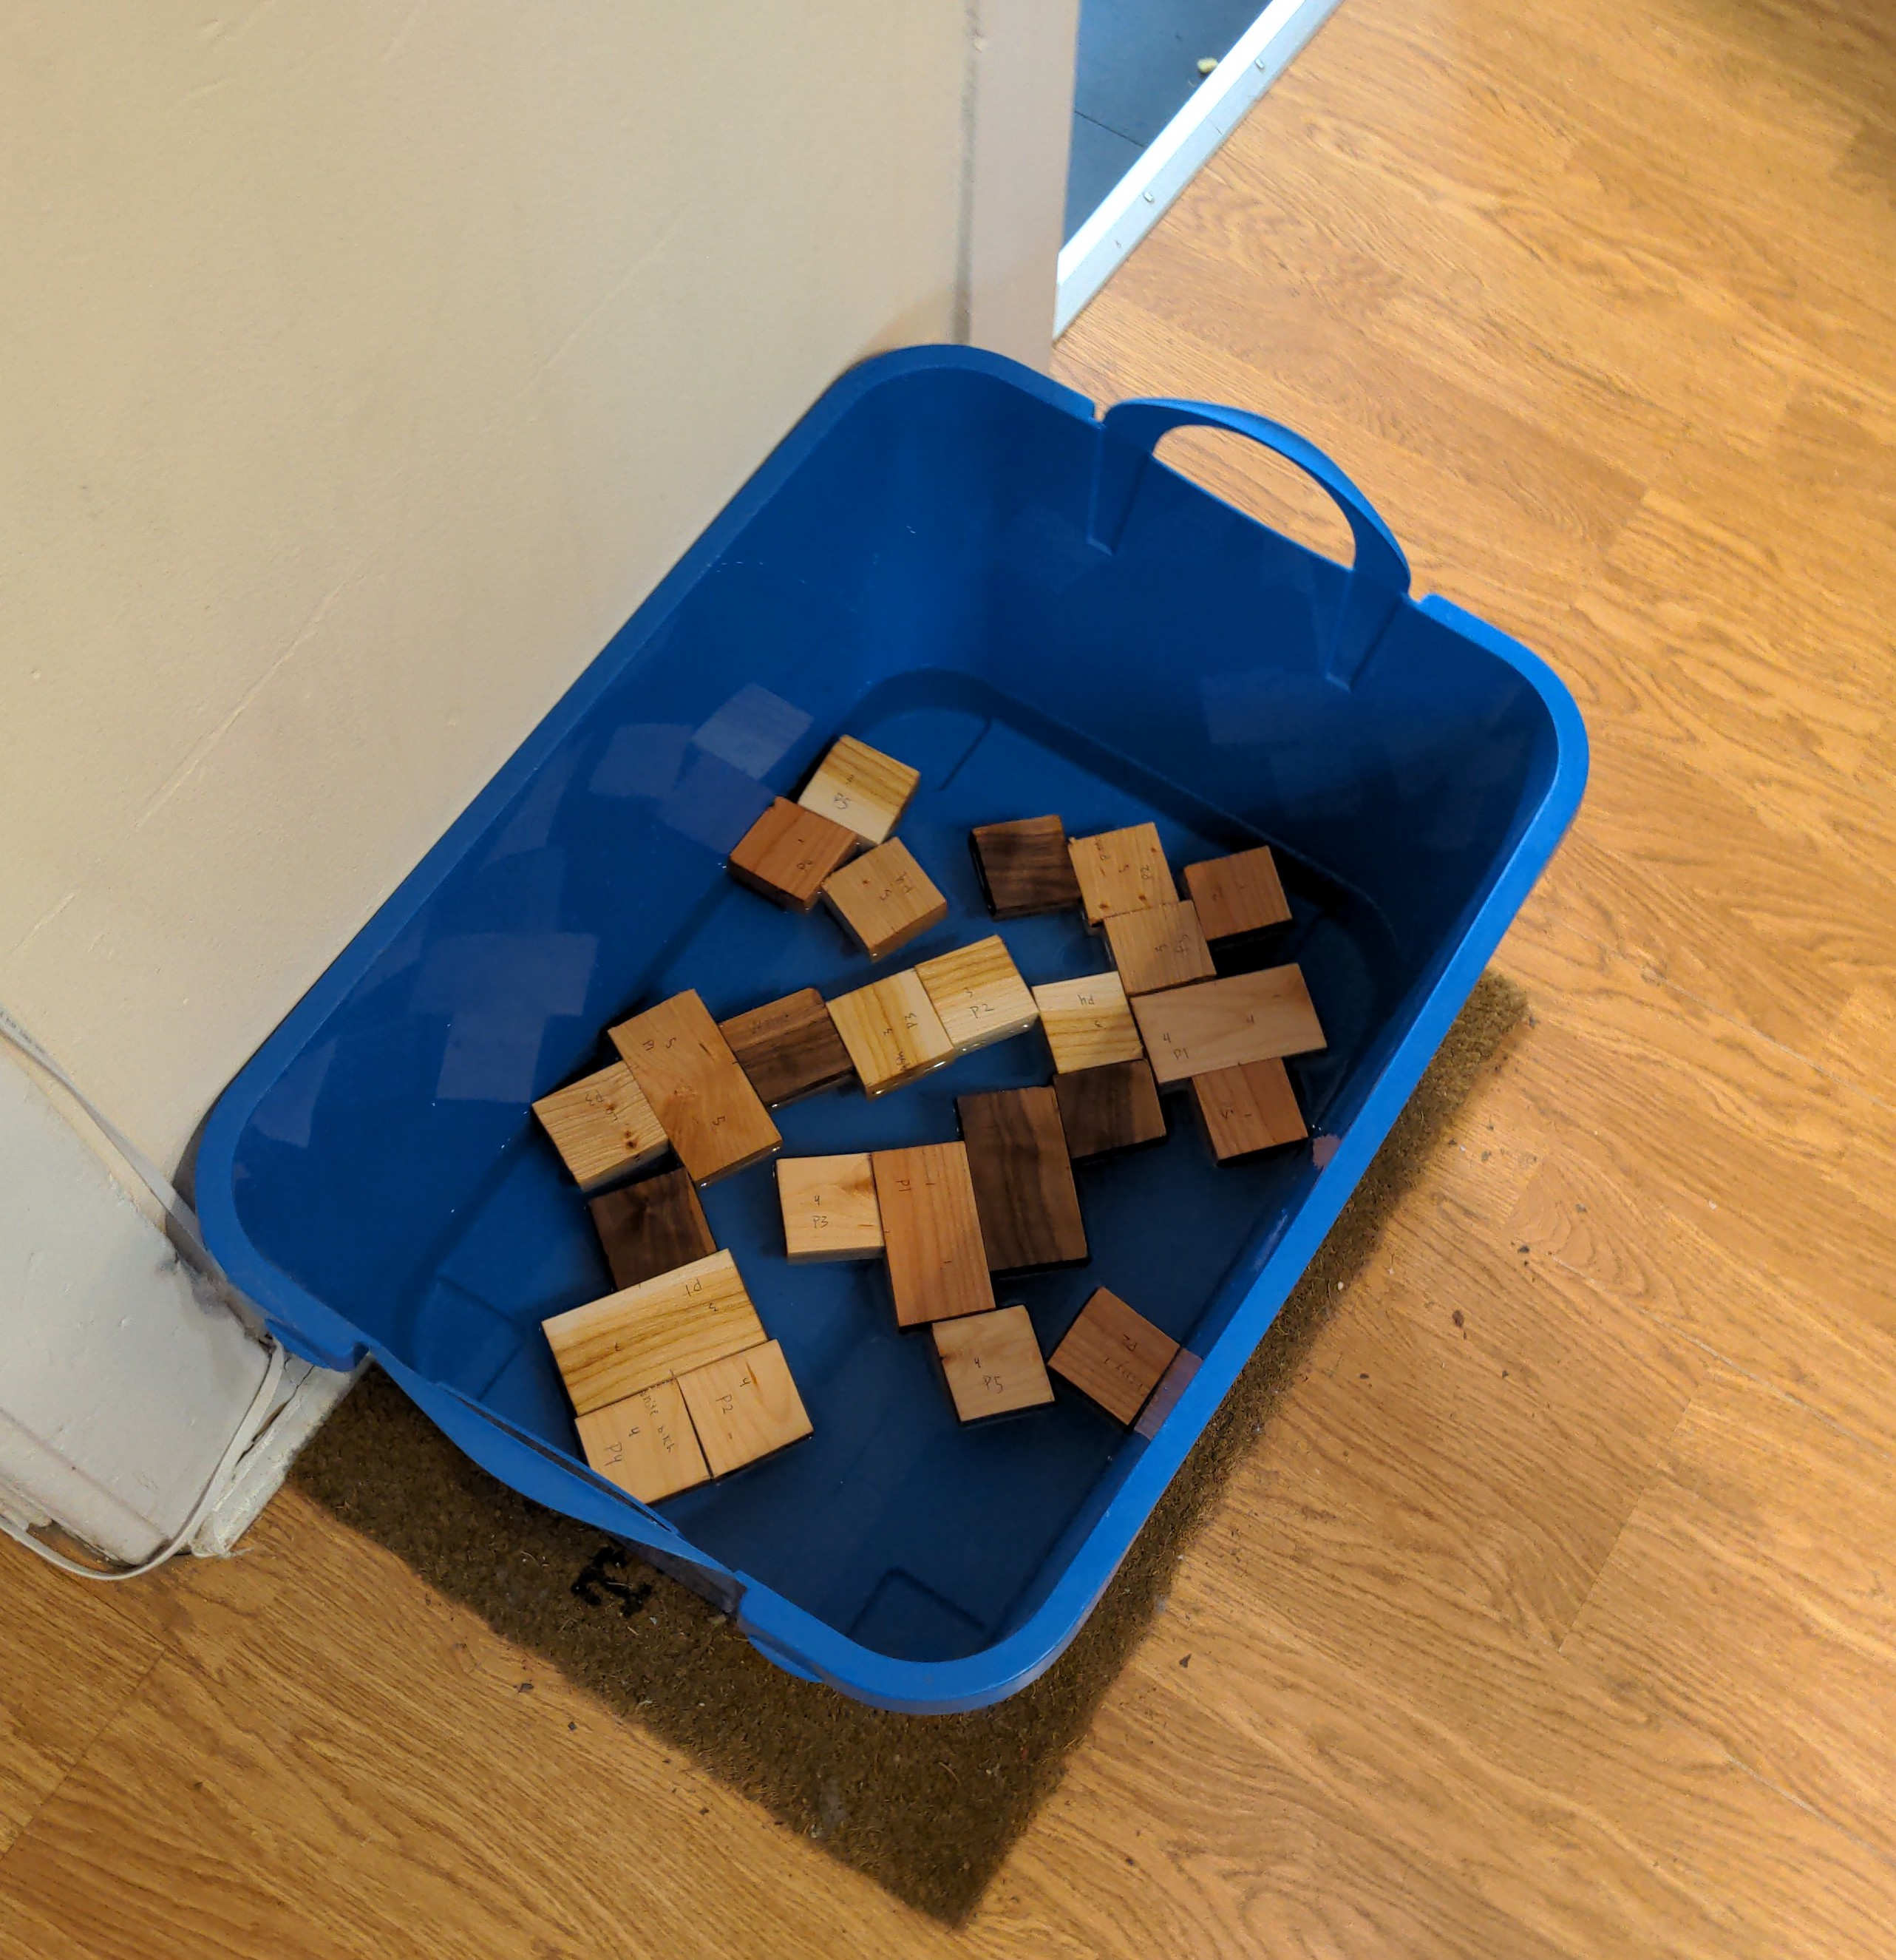
\includegraphics[width=0.5\linewidth]{wood_samples} 

}

\caption{Experiment data collection}\label{fig:unnamed-chunk-2}
\end{figure}

Summary of experiment-

We used samples of Ash, Cherry, Pine, Walnut and White Birch, with each
four replicates. Each replicate was a square 2'' wood block. All of the
specimens were left in the same bucket of water for 24 hours. Their
weight was taken before and after the 24 hour time period. Because of
sourcing constraints, each piece of wood is from the same plank, meaning
that they might not actually be independent. Another obstacle we had was
the amount of time. We let the wood sit in the water for 24 hours before
measuring it's mass again.

\hypertarget{results-and-discussion}{%
\subsection{Results and Discussion}\label{results-and-discussion}}

\begin{Shaded}
\begin{Highlighting}[]
\NormalTok{dat }\OtherTok{=} \FunctionTok{read\_csv}\NormalTok{(}\StringTok{\textquotesingle{}newdata.csv\textquotesingle{}}\NormalTok{)}
\end{Highlighting}
\end{Shaded}

\begin{verbatim}
## 
## -- Column specification --------------------------------------------------------
## cols(
##   Wood_Type = col_character(),
##   Replicate_No = col_double(),
##   Mass_Before = col_double(),
##   Mass_After = col_double(),
##   Percent_Increase = col_double(),
##   Average_Per_Type = col_double()
## )
\end{verbatim}

\begin{Shaded}
\begin{Highlighting}[]
\FunctionTok{ggplot}\NormalTok{(dat) }\SpecialCharTok{+}
  \FunctionTok{geom\_point}\NormalTok{( }\FunctionTok{aes}\NormalTok{(}\AttributeTok{x =}\NormalTok{ Wood\_Type, }\AttributeTok{y =}\NormalTok{ Percent\_Increase)) }\SpecialCharTok{+}
  \FunctionTok{geom\_hline}\NormalTok{(}\FunctionTok{aes}\NormalTok{(}\AttributeTok{yintercept =} \FunctionTok{mean}\NormalTok{(dat}\SpecialCharTok{$}\NormalTok{Percent\_Increase)), }\AttributeTok{color =} \StringTok{"steelblue"}\NormalTok{) }\SpecialCharTok{+}
  \FunctionTok{ggtitle}\NormalTok{(}\StringTok{\textquotesingle{}Percent Increase in Mass for Water Soaked Wood\textquotesingle{}}\NormalTok{) }\SpecialCharTok{+}
  \FunctionTok{xlab}\NormalTok{(}\StringTok{\textquotesingle{}Wood Type\textquotesingle{}}\NormalTok{) }\SpecialCharTok{+}
  \FunctionTok{ylab}\NormalTok{(}\StringTok{\textquotesingle{}Percent Increase in Mass after 24 Hours\textquotesingle{}}\NormalTok{)}
\end{Highlighting}
\end{Shaded}

\includegraphics{Final_Project_files/figure-latex/unnamed-chunk-3-1.pdf}

\begin{Shaded}
\begin{Highlighting}[]
\NormalTok{dat }\OtherTok{\textless{}{-}}\NormalTok{ dat }\SpecialCharTok{\%\textgreater{}\%}
  \FunctionTok{mutate}\NormalTok{(}\AttributeTok{Wood\_Type =} \FunctionTok{case\_when}\NormalTok{(Wood\_Type }\SpecialCharTok{==} \StringTok{"Cherry"} \SpecialCharTok{\textasciitilde{}} \DecValTok{1}\NormalTok{,}
\NormalTok{                                   Wood\_Type }\SpecialCharTok{==} \StringTok{"Walnut"} \SpecialCharTok{\textasciitilde{}} \DecValTok{2}\NormalTok{,}
\NormalTok{                                   Wood\_Type }\SpecialCharTok{==} \StringTok{"Ash"} \SpecialCharTok{\textasciitilde{}} \DecValTok{3}\NormalTok{,}
\NormalTok{                                   Wood\_Type }\SpecialCharTok{==} \StringTok{"White Birch"} \SpecialCharTok{\textasciitilde{}} \DecValTok{4}\NormalTok{,}
\NormalTok{                                   Wood\_Type }\SpecialCharTok{==} \StringTok{"Pine"} \SpecialCharTok{\textasciitilde{}} \DecValTok{5}\NormalTok{)) }\SpecialCharTok{\%\textgreater{}\%}
  \FunctionTok{select}\NormalTok{(Percent\_Increase, Wood\_Type)}
\NormalTok{dat}\SpecialCharTok{$}\NormalTok{Wood\_Type }\OtherTok{=} \FunctionTok{as.factor}\NormalTok{(dat}\SpecialCharTok{$}\NormalTok{Wood\_Type)}

\NormalTok{fit }\OtherTok{\textless{}{-}} \FunctionTok{aov}\NormalTok{(Percent\_Increase }\SpecialCharTok{\textasciitilde{}}\NormalTok{ Wood\_Type, }\AttributeTok{data =}\NormalTok{ dat)}
\FunctionTok{summary}\NormalTok{(fit)}
\end{Highlighting}
\end{Shaded}

\begin{verbatim}
##             Df Sum Sq Mean Sq F value   Pr(>F)    
## Wood_Type    4  567.7  141.93   16.65 2.16e-05 ***
## Residuals   15  127.8    8.52                     
## ---
## Signif. codes:  0 '***' 0.001 '**' 0.01 '*' 0.05 '.' 0.1 ' ' 1
\end{verbatim}

Our P-value is 2.16e-05, which is significantly less than
\(\alpha = 0.01\). There exists significant evidence that we can reject
\(H_0\), that is, the mean moisture content is different among types.

With a p-value of less than 0.0001, there is strong evidence against the
null hypothesis. We reject that each wood type absorbs the same amount
of water.

\begin{Shaded}
\begin{Highlighting}[]
\FunctionTok{TukeyHSD}\NormalTok{(fit, }\AttributeTok{conf.level =} \FloatTok{0.99}\NormalTok{)}
\end{Highlighting}
\end{Shaded}

\begin{verbatim}
##   Tukey multiple comparisons of means
##     99% family-wise confidence level
## 
## Fit: aov(formula = Percent_Increase ~ Wood_Type, data = dat)
## 
## $Wood_Type
##           diff         lwr       upr     p adj
## 2-1  -1.288424  -9.3982186  6.821371 0.9688287
## 3-1   6.966107  -1.1436881 15.075902 0.0291177
## 4-1  10.203374   2.0935796 18.313169 0.0014185
## 5-1  -3.989207 -12.0990023  4.120587 0.3430638
## 3-2   8.254530   0.1447356 16.364325 0.0087275
## 4-2  11.491798   3.3820033 19.601593 0.0004435
## 5-2  -2.700784 -10.8105786  5.409011 0.6904564
## 4-3   3.237268  -4.8725271 11.347063 0.5377809
## 5-3 -10.955314 -19.0651090 -2.845519 0.0007161
## 5-4 -14.192582 -22.3023767 -6.082787 0.0000450
\end{verbatim}

Using Tukey's HSD and an \(\alpha = 0.01\), we can see exactly which
wood types differ from each other.

\hypertarget{todo}{%
\section{TODO}\label{todo}}

UPDATE TO REFLECT ALPHA = 0.01 In this case, the p-values suggest a
difference in water absorption for wood 3 and 1, wood 4 and 1, wood 3
and 2, wood 4 and 2, wood 5 and 3, and wood 5 and 4.

\hypertarget{todo-1}{%
\section{TODO}\label{todo-1}}

Check model assumptions, normality of residuals, assumption of equal
variance \ldots{}

\hypertarget{conclusion}{%
\subsection{Conclusion}\label{conclusion}}

\hypertarget{todo-2}{%
\section{TODO}\label{todo-2}}

Elaborate on how what we learned can be used in engineering
applications? What would we do different? Is there a difference
experiment design that would have given more insight on this process
(maybe blocking or two way factorial)? How can researchers replicate?

\hypertarget{style-and-organization}{%
\subsection{Style and Organization}\label{style-and-organization}}

\hypertarget{todo-3}{%
\section{TODO}\label{todo-3}}

Make sure project knits well into PDF and all code is displayed
according to milestone.

\end{document}
